\documentclass{article}\usepackage[]{graphicx}\usepackage[]{color}
%% maxwidth is the original width if it is less than linewidth
%% otherwise use linewidth (to make sure the graphics do not exceed the margin)
\makeatletter
\def\maxwidth{ %
  \ifdim\Gin@nat@width>\linewidth
    \linewidth
  \else
    \Gin@nat@width
  \fi
}
\makeatother

\definecolor{fgcolor}{rgb}{0.345, 0.345, 0.345}
\newcommand{\hlnum}[1]{\textcolor[rgb]{0.686,0.059,0.569}{#1}}%
\newcommand{\hlstr}[1]{\textcolor[rgb]{0.192,0.494,0.8}{#1}}%
\newcommand{\hlcom}[1]{\textcolor[rgb]{0.678,0.584,0.686}{\textit{#1}}}%
\newcommand{\hlopt}[1]{\textcolor[rgb]{0,0,0}{#1}}%
\newcommand{\hlstd}[1]{\textcolor[rgb]{0.345,0.345,0.345}{#1}}%
\newcommand{\hlkwa}[1]{\textcolor[rgb]{0.161,0.373,0.58}{\textbf{#1}}}%
\newcommand{\hlkwb}[1]{\textcolor[rgb]{0.69,0.353,0.396}{#1}}%
\newcommand{\hlkwc}[1]{\textcolor[rgb]{0.333,0.667,0.333}{#1}}%
\newcommand{\hlkwd}[1]{\textcolor[rgb]{0.737,0.353,0.396}{\textbf{#1}}}%

\usepackage{framed}
\makeatletter
\newenvironment{kframe}{%
 \def\at@end@of@kframe{}%
 \ifinner\ifhmode%
  \def\at@end@of@kframe{\end{minipage}}%
  \begin{minipage}{\columnwidth}%
 \fi\fi%
 \def\FrameCommand##1{\hskip\@totalleftmargin \hskip-\fboxsep
 \colorbox{shadecolor}{##1}\hskip-\fboxsep
     % There is no \\@totalrightmargin, so:
     \hskip-\linewidth \hskip-\@totalleftmargin \hskip\columnwidth}%
 \MakeFramed {\advance\hsize-\width
   \@totalleftmargin\z@ \linewidth\hsize
   \@setminipage}}%
 {\par\unskip\endMakeFramed%
 \at@end@of@kframe}
\makeatother

\definecolor{shadecolor}{rgb}{.97, .97, .97}
\definecolor{messagecolor}{rgb}{0, 0, 0}
\definecolor{warningcolor}{rgb}{1, 0, 1}
\definecolor{errorcolor}{rgb}{1, 0, 0}
\newenvironment{knitrout}{}{} % an empty environment to be redefined in TeX

\usepackage{alltt}
% section added by EE227AT HW1
\usepackage{fullpage,marginnote,caption}
%\usepackage{graphicx,psfrag}

%\usepackage{nips01e}
\usepackage{amsfonts}
%\usepackage{harvard}
\usepackage{amsmath}
\usepackage{fullpage}
%\usepackage[dutch]{babel}
%\usepackage[subnum]{cases}
\usepackage{amssymb}
%\usepackage{psfrag}
\usepackage{graphicx}
\usepackage{fancyhdr,color}
%\usepackage{mcode}
\newcommand{\red}[1]{\textcolor{red}{#1}}
\newcommand{\green}[1]{\textcolor{green}{#1}}
\usepackage{enumerate}



%\newtheorem{remark}{Remark}
\newtheorem{lemma}{Lemma}
\newtheorem{fact}{Fact}
\usepackage{natbib}
\usepackage[unicode=true]{hyperref}
\usepackage{geometry}
\geometry{tmargin=1in,bmargin=1in,lmargin=1in,rmargin=1in}
% The geometry package allows for easy page formatting.
\newcommand{\red}[1]{\textcolor{red}{#1}}
\newcommand{\green}[1]{\textcolor{green}{#1}}
\usepackage[procnames]{listings}
\usepackage{color}

\definecolor{keywords}{RGB}{255,0,90}
\definecolor{comments}{RGB}{0,0,113}
\definecolor{red}{RGB}{160,0,0}
\definecolor{green}{RGB}{0,150,0}
 
\lstset{language=Python,%
    %basicstyle=\color{red},
    breaklines=true,%
    morekeywords={matlab2tikz},
    keywordstyle=\color{blue},%
    morekeywords=[2]{1}, keywordstyle=[2]{\color{black}},
    identifierstyle=\color{black},%
    stringstyle=\color{mylilas},
    commentstyle=\color{mygreen},%
    showstringspaces=false,%without this there will be a symbol in the places where there is a space
    numbers=left,%
    numberstyle={\tiny \color{black}},% size of the numbers
    numbersep=9pt, % this defines how far the numbers are from the text
    emph=[1]{for,end,break},emphstyle=[1]\color{red}, %some words to emphasise
    %emph=[2]{word1,word2}, emphstyle=[2]{style},    
}
     
        
\usepackage{hyperref}
\usepackage{filecontents}
\begin{filecontents}{\job5.bib}
@article{greenwade93,
    author  = "George D. Greenwade",
    title   = "The {C}omprehensive {T}ex {A}rchive {N}etwork ({CTAN})",
    year    = "1993",
    journal = "TUGBoat",
    volume  = "14",
    number  = "3",
    pages   = "342--351"
}
@book{anselin2013spatial,
  title={Spatial econometrics: methods and models},
  author={Anselin, Luc},
  volume={4},
  year={2013},
  publisher={Springer Science \& Business Media}
}
\end{filecontents}

\usepackage{natbib}
\IfFileExists{upquote.sty}{\usepackage{upquote}}{}
\begin{document} 
\title{UrbanSIM Review}
\author{Danqing Zhang}
\date{\today{}}

\maketitle




\tableofcontents



\section{Household location choice model}

\subsection{Household table}








\subsection{First step:household relocation model and transition model}
\subsubsection{Household relocation model}
\begin{itemize}
\item{code location}\\
models.py (urbansim\_defaults), settings.yaml\\
\item{model explanation}\\
simple rate-based model reallocating 5\% of households annually\\
\item{output}\\
they lose their building id and are reassigned by the hlcm (?)
\end{itemize}

\subsubsection{Household transition model}
\begin{itemize}
\item{code location}\\
models.py (urbansim\_defaults), settings.yaml
\item{model explanation}\\
generates new households based on control totals (?)\\
does does it take care of aging, household formation, etc as well?\\
\item{output}
\end{itemize}





\subsection{Household location choice model}
\subsubsection{Model Explanation}
\subsubsection{Input and output}
\begin{lstlisting}
@orca.step('hlcm_owner_estimate')
def hlcm_owner_estimate(households, residential_units, unit_aggregations):
    return utils.lcm_estimate("hlcm_owner.yaml", households, "unit_id",residential_units, unit_aggregations)
\end{lstlisting}

From the code above, we can see that, households orca.table and residential\_units orca.table, as well as the unit\_aggregations orca.injective are the inputs.


\subsubsection{LCM\_estimate function from urbansim.utils}
\begin{enumerate}

\item{Here we need to make this clearer by comparision}\\

\begin{itemize}
\item{function}\\
Signature: utils.lcm\_estimate(cfg, choosers, chosen\_fname, buildings, join\_tbls)\\
where cfg refers to the yaml file;\\
chooser refers to either households or developers orca.table;\\
chosen\_fanme refers to the name of the column (present in choosers) which contains the ids that identify the chosen alternatives;\\
buildings refers to either the residential\_units or commercial\_units;\\
join\_tbls refers to orca.injective (A list of land use dataframes to give neighborhood info around the buildings will be joined to the buildings using existing broadcasts)\\
\item{calling the function}\\
cfg:"hlcm\_owner.yaml"\\
chooser orca.table:households\\
chosen\_fname:"unit\_id"\\
buildings:residential\_units\\
join\_tbls:unit\_aggregations=buildings,nodes,logsums\\
\end{itemize}


\item{Then how will the input be processed to get the output?}
\begin{lstlisting}
def lcm_estimate(cfg, choosers, chosen_fname, buildings, join_tbls):
    cfg = misc.config(cfg)
    choosers = to_frame(choosers, [], cfg, additional_columns=[chosen_fname])
    alternatives = to_frame(buildings, join_tbls, cfg)
    return yaml_to_class(cfg).fit_from_cfg(choosers,chosen_fname,alternatives,cfg)
\end{lstlisting}

\end{enumerate}


\subsubsection{How model is built?}

The below table shows where each variables comes from. And the idea is that:now units are replacing units in updated version.But currently based on what the \\

\begin{table}[]
\centering
\caption{My caption}
\label{my-label}
\begin{tabular}{|l|l|}
\hline
\textbf{var}                               & \textbf{orca.table} \\ \hline
np.log1p(residential\_price)               & buildings           \\ \hline
np.log1p(sqft\_per\_unit)                  & buildings           \\ \hline
ave\_lot\_size\_per\_unit                  & nodes               \\ \hline
ave\_income                                & nodes               \\ \hline
persons                                    & households          \\ \hline
ave\_hhsize                                & nodes               \\ \hline
white/black/hisp/asian                     & households          \\ \hline
pct\_white/pct\_black/pct\_hisp/pct\_asian & nodes               \\ \hline
jobs                                       & nodes               \\ \hline
autoPeakTotal                              & logsums             \\ \hline
transitPeakTotal                           & logsums             \\ \hline
autoOffPeakRetail                          & logsums             \\ \hline
\end{tabular}
\end{table}


\subsubsection{How is filter built and how is segmented discrete choice model built?}

\red{hownrent} is a column that indicate the household is the owner of the unit of the household is a renter of the unit.\\
\begin{lstlisting}
choosers_fit_filters:
- hownrent == 1

choosers_predict_filters:
- hownrent == 1
\end{lstlisting}


\subsubsection{Urbansim\_defaults}
Here many basic models are defined\\
And they call below puthon packages from urbansim:\\
\begin{lstlisting}
from urbansim.models import RegressionModel, SegmentedRegressionModel, \
    MNLDiscreteChoiceModel, SegmentedMNLDiscreteChoiceModel, \
    GrowthRateTransition, transition
from urbansim.models.supplydemand import supply_and_demand
from urbansim.developer import sqftproforma, developer
from urbansim.utils import misc
\end{lstlisting}





\section{Cost Function Procedure for Discrete Choice Model}

\subsection{Current Model}

\subsection{Setps}


This task consists of three steps:\\

\begin{itemize}
\item{construct a new dataframe accommodating needed variables from households table, residential\_units table, and the the units\_aggregations orca injective, consisting of three dataframes}
\item{regression residential\_price on other explanatory variables, and get residual as a pandas series, and add it as a column of the building orca.table(strange, why price is the at building level instead of units\_level?)}
\item{create a new yaml file and a new orca step for the new hlcm model with residual variables.}
\end{itemize}



\vsapce{20cm}



\section{Data Source}
\subsection{H5 file}


\begin{lstlisting}
#Putting tables in the HDF5 file
store = pd.HDFStore(h5_path)
store['parcels'] = parcels # http://urbansim.org/Documentation/Parcel/ParcelTable
store['buildings'] = buildings # http://urbansim.org/Documentation/Parcel/BuildingsTable
store['households'] = hh # http://urbansim.org/Documentation/Parcel/HouseholdsTable
store['jobs'] = jobs # http://urbansim.org/Documentation/Parcel/JobsTable
store['zones'] = zones # http://urbansim.org/Documentation/Parcel/ZonesTable
store.close()
\end{lstlisting}


\begin{lstlisting}
@orca.table('jobs', cache=True)
def jobs(store):
    # nets = store['nets']
    ###go from establishments to jobs
    # df = nets.loc[np.repeat(nets.index.values, nets.emp11.values)]\
        # .reset_index()
    # df.index.name = 'job_id'
    df = store['jobs']
    return df
\end{lstlisting}





\section{Data Source}
Where can I get the data?
From "2015\_06\_01\_bayarea\_v3.h5", we can get "parcels","buildings","households","jobs" and "zones".Other tables are loaded in datasources.py file from local csv files from local data folder.\\
\\
datasources.py is used to load local data into orca table.Then varibales.py is used to generate new columns of existent orca tables.\\

\section{Setting, neighorhood\_vars, price\_vars}


\section{Hedonic Regression Model}

\subsection{Model Basics}
Note simple linear regression cannot be done within urbansim modules.We need statmodels to conduct regression.\\

\begin{itemize}
\item{Background in urbansim\_utils}\\
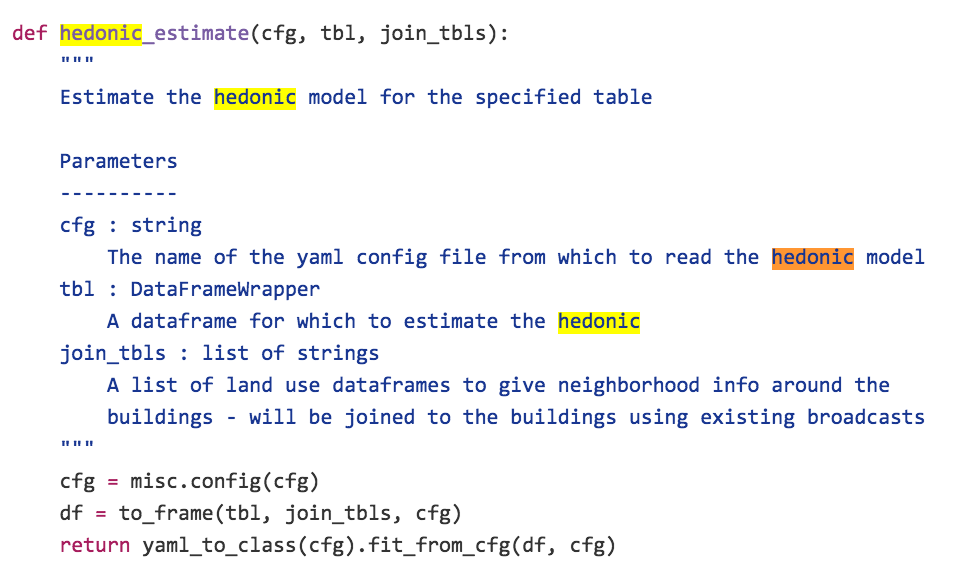
\includegraphics[width=10cm]{2.png}
\item{rrh.yaml}\\

\begin{lstlisting}
name: rrh

model_type: regression

fit_filters:
- price_sqft > 0.5
- price_sqft < 7

predict_filters: null

model_expression: np.log(price_sqft) ~ np.log1p(sqft_per_unit) + ave_lot_size_per_unit
    + ave_income  + pct_black + pct_hisp + pct_asian + pct_renters + population +
    autoPeakTotal + transitPeakTotal + autoOffPeakRetail + jobs

ytransform: np.exp

fitted: true
\end{lstlisting}

\item{First step:create rrh\_simulate as an orca "step" in models.py file}\\
from urbansim\_defaults import utils, and here call the utils.hedonic\_estimate function in urbansim\_utils package\\
\red{hedonic\_estimate is a function in urbansim\_utils, that }\\
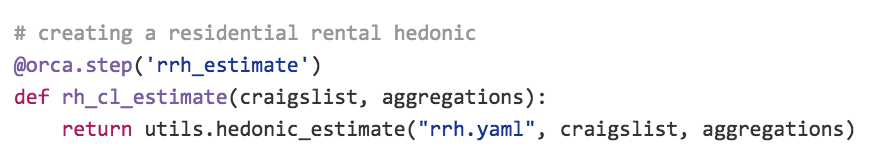
\includegraphics[width=10cm]{1.png}
\item{Second step:call rrh\_simulate step in estimation.py file and simulation.py file,since if you want to have simulation result, the first step is estimation of parameters, both for hedonic regression and MNL Discrete Choice Models}\\
\begin{lstlisting}
import time
import models
import pandas as pd
import orca

orca.run([
    "neighborhood_vars",         # accessibility variables
    "rsh_estimate"               # residential sales hedonic
    "rrh_estimate"               # residential rental hedonic
    #"rsh_simulate",
    #"hlcm_estimate"               # household lcm
])
\end{lstlisting}
\end{itemze}

\subsection{Change models}
To save variations, create a new yaml file and run this to register it(create orca step for this specific hedonic regression)\\
The coefficient can be stored or can be printed out, as below:

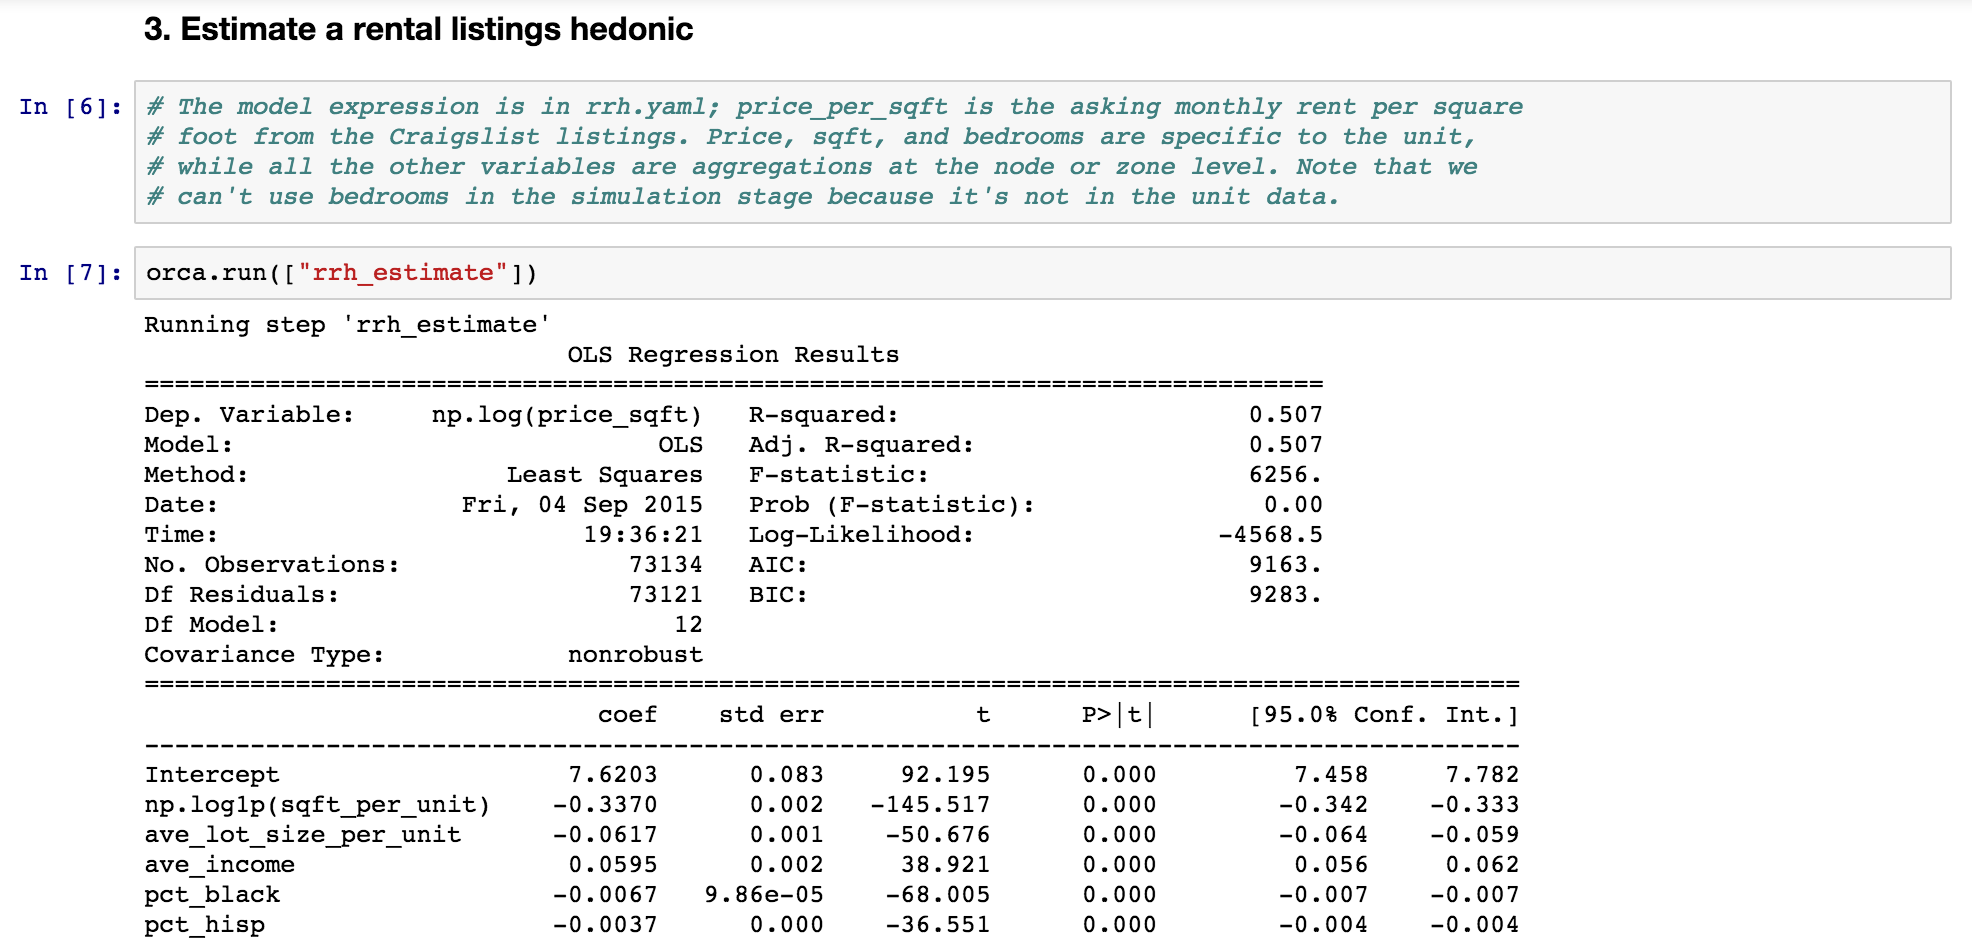
\includegraphics[width=10cm]{3.png}
\subsubsection{We package the estimation step as an orca step, so that we can call them sequentially in orca run}
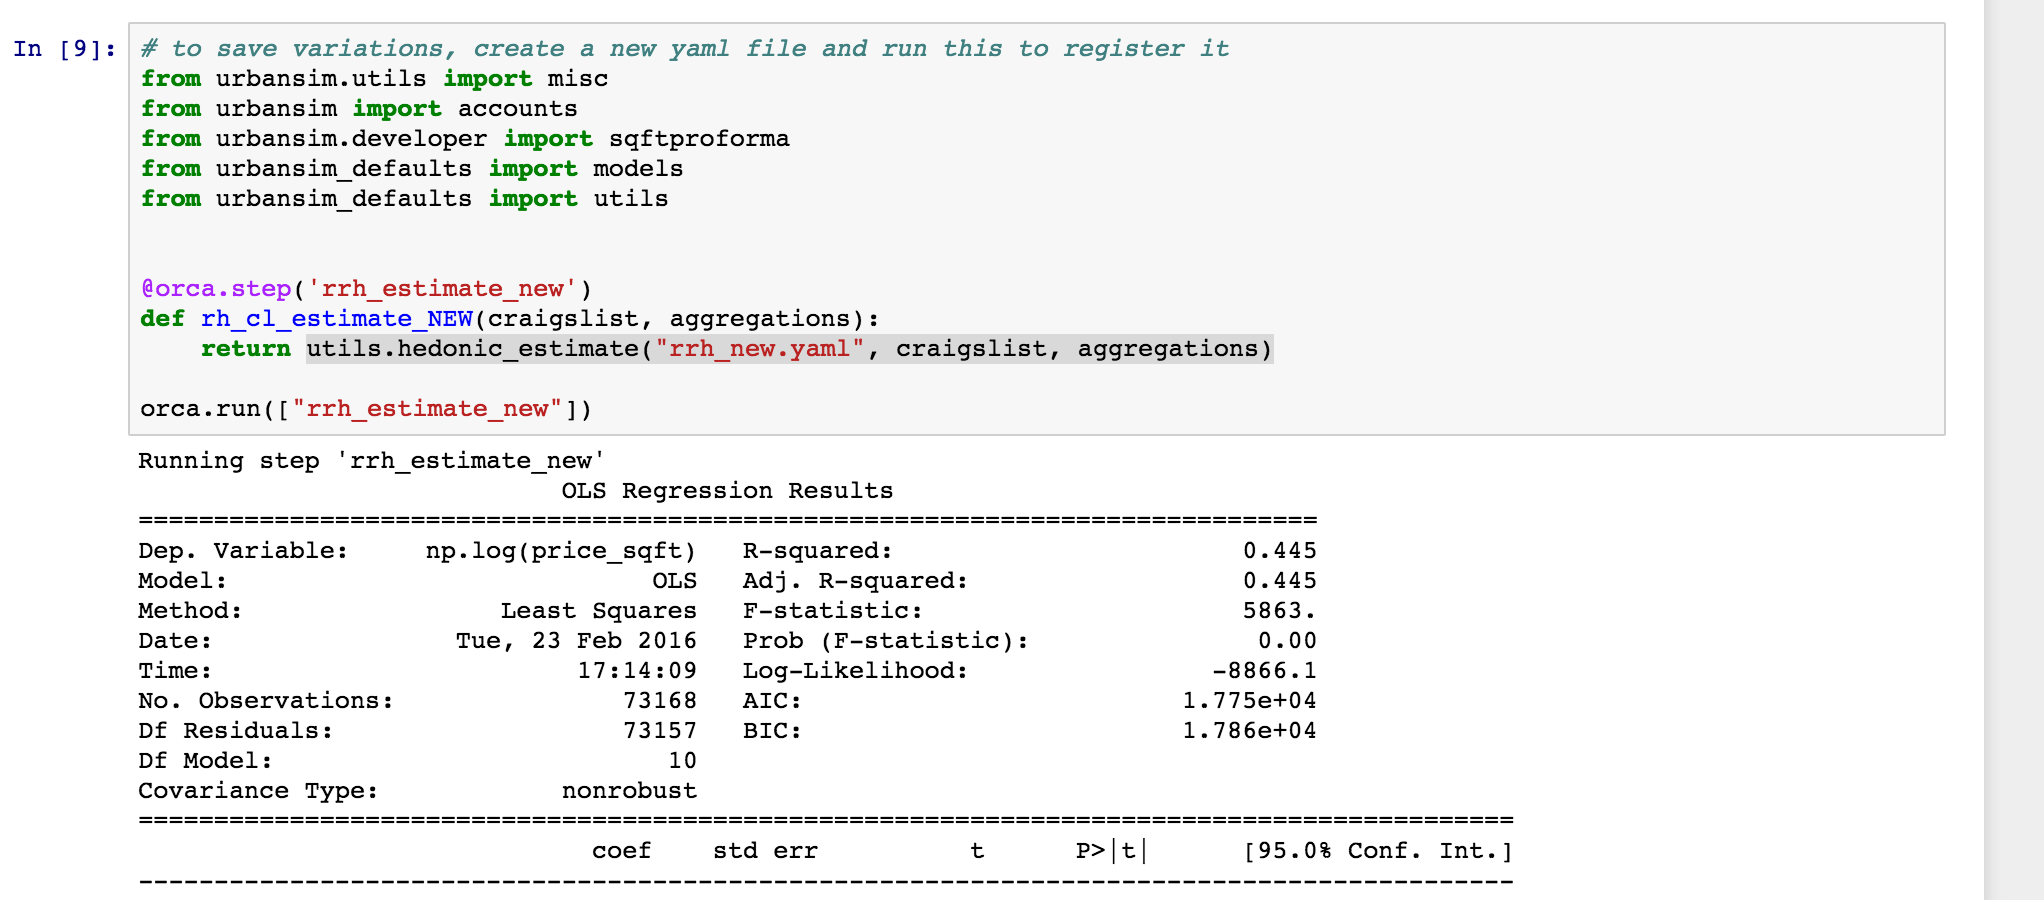
\includegraphics[width=10cm]{4.png}

\subsubsection{But we can decompose it to get the estimation function that directly gives us the regression result}
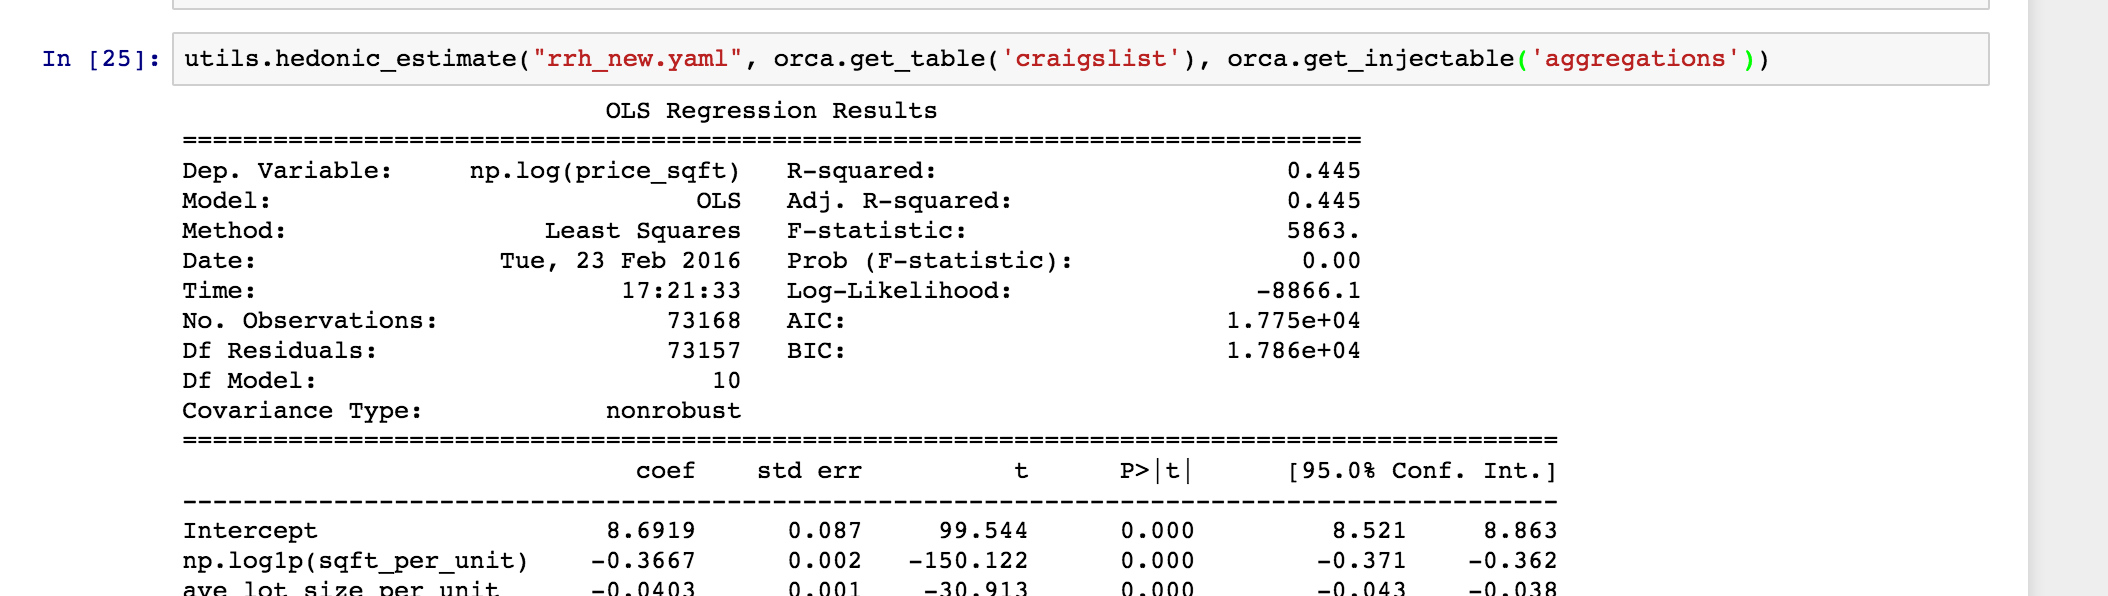
\includegraphics[width=10cm]{5.png}

\subsubsection{What is aggregations? how to get them?}
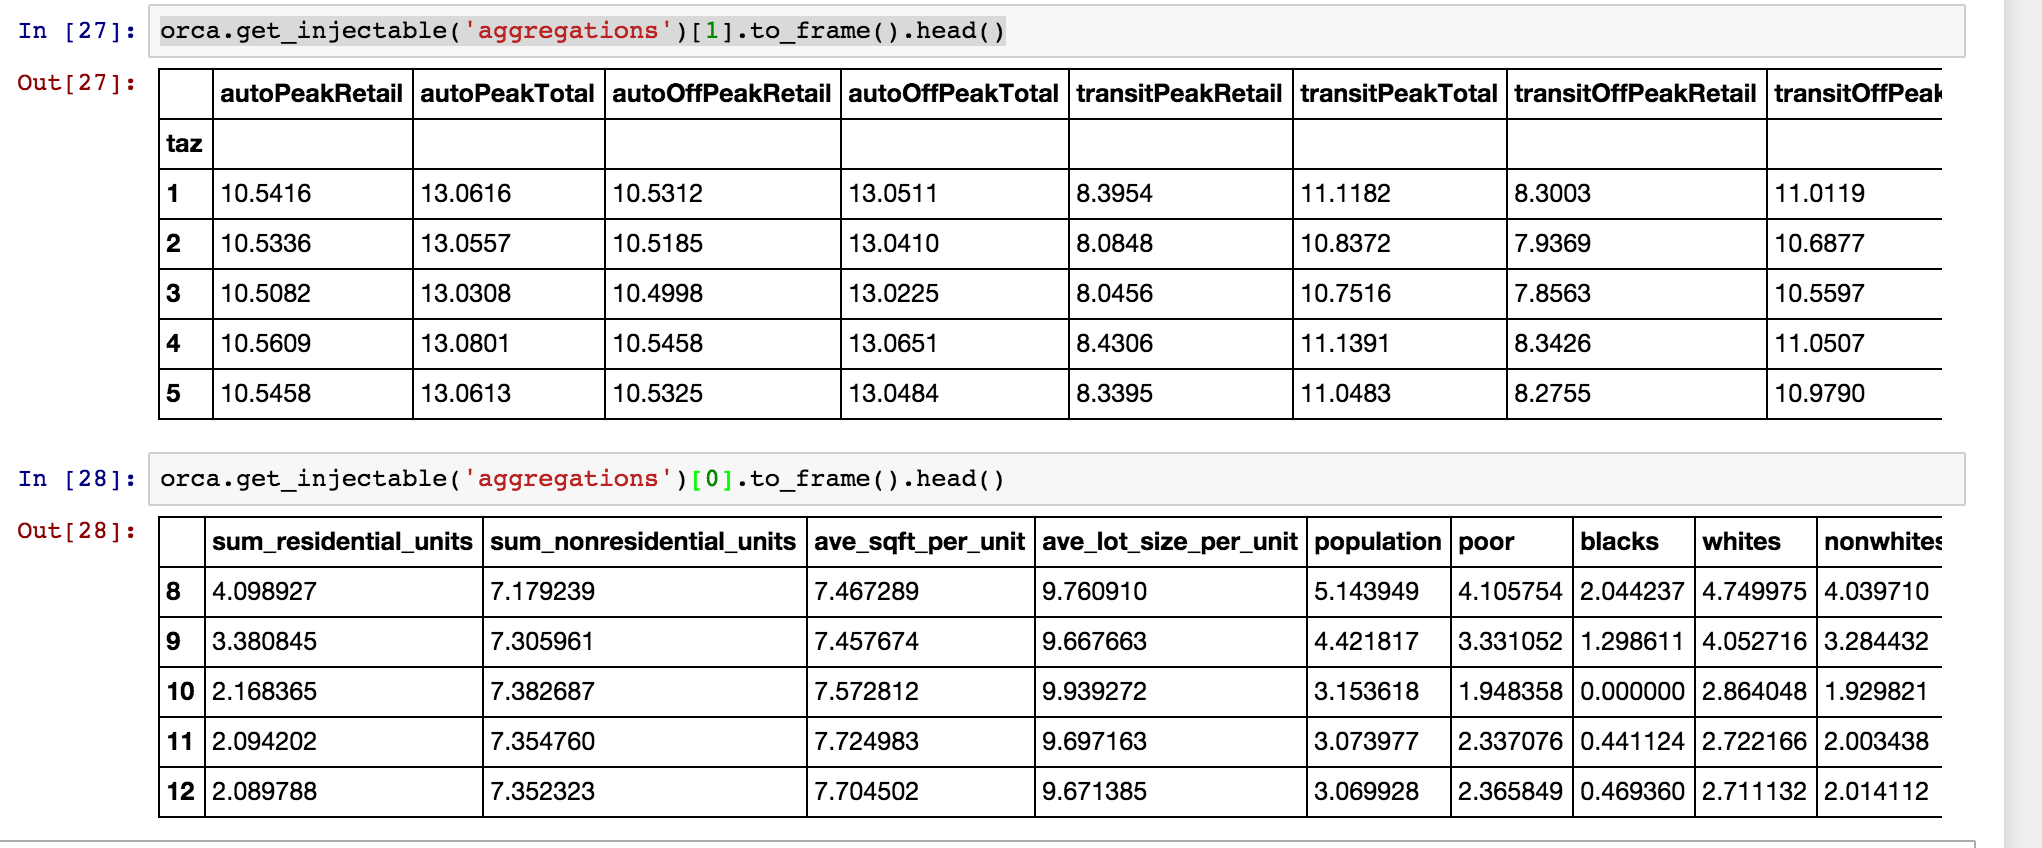
\includegraphics[width=10cm]{6.png}\\
There must be some code like this for aggregation injectable.\\
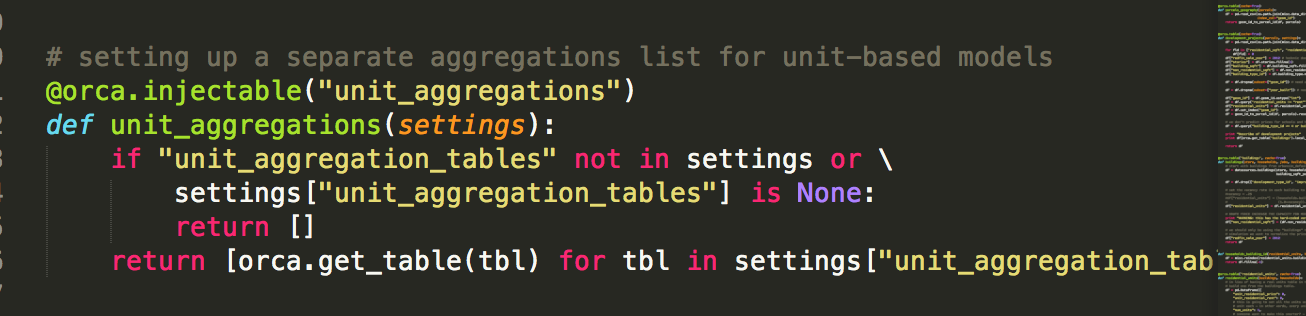
\includegraphics[width=10cm]{7.png}\\

It can be concluded that :
\begin{itemize}
\item{orca.injectable is a list of orca.table}
\item{orca.table}
\item{orca.column}\\
And from urbansim.utils import misc, since the orca.column step will have to use this function\\
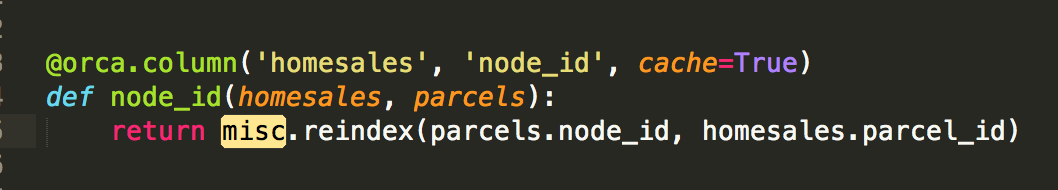
\includegraphics[width=10cm]{8.png}\\

\begin{lstlisting}
Signature: misc.reindex(series1, series2)
Source:
def reindex(series1, series2):
    """
    This reindexes the first series by the second series.  This is an extremely
    common operation that does not appear to  be in Pandas at this time.
    If anyone knows of an easier way to do this in Pandas, please inform the
    UrbanSim developers.

    The canonical example would be a parcel series which has an index which is
    parcel_ids and a value which you want to fetch, let's say it's land_area.
    Another dataset, let's say of buildings has a series which indicate the
    parcel_ids that the buildings are located on, but which does not have
    land_area.  If you pass parcels.land_area as the first series and
    buildings.parcel_id as the second series, this function returns a series
    which is indexed by buildings and has land_area as values and can be
    added to the buildings dataset.

    In short, this is a join on to a different table using a foreign key
    stored in the current table, but with only one attribute rather than
    for a full dataset.

    This is very similar to the pandas "loc" function or "reindex" function,
    but neither of those functions return the series indexed on the current
    table.  In both of those cases, the series would be indexed on the foreign
    table and would require a second step to change the index.
    """

    # turns out the merge is much faster than the .loc below
    df = pd.merge(pd.DataFrame({"left": series2}),
                  pd.DataFrame({"right": series1}),
                  left_on="left",
                  right_index=True,
                  how="left")
    return df.right
File:      ~/anaconda/lib/python2.7/site-packages/urbansim-3.1.dev0-py2.7.egg/urbansim/utils/misc.py
Type:      function
\end{lstlisting}
\end{itemize}




\section{Hedonic Simulation Model}







\section{lcm-estimate}


\section{lcm-simulation}


\section{simple-relocation}

\subsection{Model basics}


\begin{lstlisting}
Signature: utils.simple_relocation(choosers, relocation_rate, fieldname)
Source:
def simple_relocation(choosers, relocation_rate, fieldname):
    """
    Run a simple rate based relocation model

    Parameters
    ----------
    tbl : DataFrameWrapper or DataFrame
        Table of agents that might relocate
    rate : float
        Rate of relocation
    location_fname : str
        The field name in the resulting dataframe to set to -1 (to unplace
        new agents)

    Returns
    -------
    Nothing
    """
    print "Total agents: %d" % len(choosers)
    _print_number_unplaced(choosers, fieldname)

    print "Assigning for relocation..."
    chooser_ids = np.random.choice(choosers.index, size=int(relocation_rate *
                                   len(choosers)), replace=False)
    choosers.update_col_from_series(fieldname,
                                    pd.Series(-1, index=chooser_ids))

    _print_number_unplaced(choosers, fieldname)
File:      ~/Google_Drive/Berkeley/research/2015Fall/bayarea_urbansim/build/bdist.macosx-10.5-x86_64/egg/urbansim_defaults/utils.py
Type:      function
\end{lstlisting}




\section{@orca.step("travel\_model\_output")}



Dolor sit amet~\citep{greenwade93}.
\bibliographystyle{plainnat}
\bibliography{\job5} 

\end{document}

